\documentclass[11pt,a4paper,twoside,openright]{book}
\usepackage[T1]{fontenc}
\usepackage{lmodern}
\usepackage{graphicx}
\usepackage{xcolor}
\definecolor{accent}{RGB}{20,50,120}
\definecolor{linkblue}{RGB}{0,70,180}
\definecolor{boxtint}{RGB}{225,235,250}
\usepackage[round,authoryear]{natbib}
\usepackage[colorlinks=true,linkcolor=linkblue,citecolor=linkblue]{hyperref}
\usepackage{titlesec}
\titleformat{\chapter}{\Huge\bfseries\color{accent}}{\thechapter}{1em}{}
\begin{document}
\frontmatter
\tableofcontents
\listoffigures
\mainmatter
\chapter{Introduction}\label{ch:intro}
Tabular foundation models are pretrained on many tables~\citep{smith2020}. See Chapter~\ref{ch:method}.
\chapter{Method}\label{ch:method}
\noindent\colorbox{boxtint}{\parbox{0.85\linewidth}{I developed the method in this chapter.}}
\begin{figure}[t]
\centering
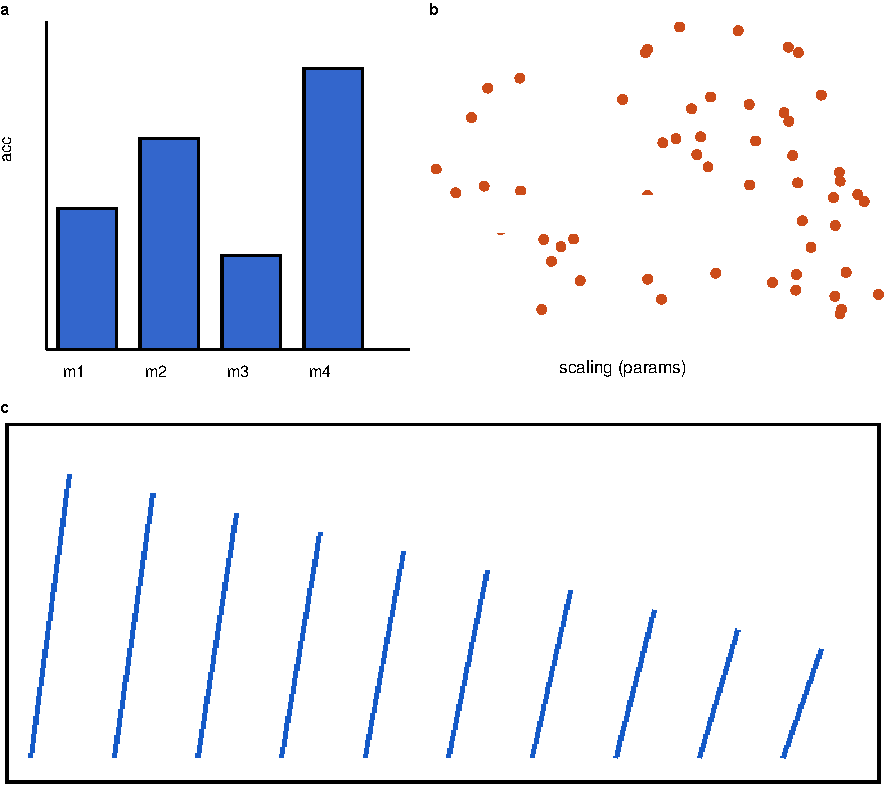
\includegraphics[width=\linewidth]{figures/fig_example.pdf}
\caption{\textbf{Accuracy rises with model size.} \textbf{a}, Accuracy per model. \textbf{b}, Scaling. \textbf{c}, Learning curves. Adapted from Fig.~2a,b and Fig.~3 of \citet{smith2020}.}
\label{fig:example}
\end{figure}
\noindent The composed figure is shown in Figure~\ref{fig:example}.
\bibliographystyle{plainnat}
\bibliography{refs}
\end{document}
